\documentclass[a4paper]{article}
\usepackage{amsmath}
\addtolength{\hoffset}{-2.25cm}
\addtolength{\textwidth}{4.5cm}
\addtolength{\voffset}{-3.25cm}
\addtolength{\textheight}{5cm}
\setlength{\parindent}{15pt}

\usepackage[unicode=true, colorlinks=false, hidelinks]{hyperref}
\usepackage[utf8]{inputenc}
\usepackage[english, russian]{babel}
\usepackage{mathtext}
\usepackage[T2A, TS1]{fontenc}
\usepackage{microtype} % Slightly tweak font spacing for aesthetics
\usepackage{amsthm, amssymb, amsmath, amsfonts, nccmath}
\usepackage{nicefrac}
\usepackage{epstopdf}
\usepackage[export]{adjustbox}
\usepackage{float} % Improved interface for floating objects
\usepackage{graphicx, multicol} % Enhanced support for graphics
\usepackage{pdfrender,xcolor}
\usepackage{breqn}
\usepackage{mathtools}
\usepackage{titling}
\usepackage{bm}
\usepackage{centernot}
\usepackage[cal=boondoxo,calscaled=.96]{mathalpha}
\usepackage{marvosym, wasysym} % More symbols
\usepackage{rotating} % Rotation tools
\usepackage{censor} % Facilities for controlling restricted text

\usepackage{fancyhdr}
\pagestyle{fancy}
\fancyhead{}\renewcommand{\headrulewidth}{0pt}
\fancyfoot[L]{}
\fancyhead{}
\fancyfoot{}
\fancyfoot[R]{\thepage}
\begin{document}
    \begin{titlepage}
   \begin{center}
       \vspace*{3cm}
       \large{САНКТ-ПЕТЕРБУРГСКИЙ ПОЛИТЕХНИЧЕСКИЙ УНИВЕРСИТЕТ}
       \vspace{0.4 cm}

       \large\textbf{Институт прикладной математики и механики}
       \vspace{0.4 cm}

       \large{Высшая школа прикладной математики и вычислительной физики}

       \vspace{3 cm}
       \normalsize\textbf{Отчет\\ по лабораторной работе №7\\ по дисциплине\\
«Математическая статистика»}
       \vfill
       \begin{flushright}
            \normalsize{Выполнил студент:\\
            Антонов Алексей\\
            группа: 3630102/80201}
            \vskip\medskipamount
            \normalsize{Проверил:

            к.ф.-м.н., доцент\\
            Баженов Александр Николаевич
            }
       \end{flushright}

       \vspace{0.8cm}


       \normalsize{Санкт-Петербург\\2021 г.}

   \end{center}
\end{titlepage}
    \tableofcontents
    \newpage
    \listoffigures
    \newpage
    \section{Постановка задачи}
Для 5 распределений:
    \begin{itemize}
        \item Нормальное распределение $N(x, 0, 1)$
        \item Распределение Коши $C(x, 0, 1)$
        \item Распределение Лапласа $L\left(x, 0, \frac{1}{\sqrt{2}}\right)$
        \item Распределение Пуассона $P(k, 10)$
        \item Равномерное распределение $U\left(x,-\sqrt{3},\sqrt{3}\right)$
    \end{itemize}
    Сгенерировать выборки размером 10, 50 и 1000 элементов.
    Построить на одном рисунке гистограмму и график плотности распределения.
    \section{Теория}
        \subsection{Рассматриваемые распределения}
            Плотности:
            \begin{itemize}
                \item Нормальное распределение
                \begin{equation}\label{eq:norm}
                    N(x,0,1)=\frac{1}{\sqrt{2\pi}}e^{-\frac{x^2}{2}}
                \end{equation}
                \item Распределение Коши
                \begin{equation}\label{eq:cauchy}
                    C(x, 0, 1)=\frac{1}{\pi}\frac{1}{x^2+1}
                \end{equation}
                \item Распределение Лапласа
                \begin{equation}\label{eq:laplace}
                    L(x,0,\frac{1}{\sqrt{2}})=\frac{1}{\sqrt{2}}e^{-\sqrt{2}|x|}
                \end{equation}
                \item Распределение Пуассона
                \begin{equation}\label{eq:poisson}
                    P(k, 10)=\frac{10^k}{k!}e^{-10}
                \end{equation}
                \item Равномерное распределение
                \begin{equation}\label{eq:uniform}
                    U(x,-\sqrt{3},\sqrt{3})=
                    \begin{cases}
                    \displaystyle\frac{1}{2\sqrt{3}}&\text{при}\;\;|x|\:\leq\sqrt{3}\\
                    \;\;\;0&\text{при}\;\;|x|\:>\sqrt{3}\\
                    \end{cases}
                \end{equation}
            \end{itemize}
        \subsection{Гистограмма}
            \subsubsection{Построение гистограммы}
                Множество значений, которое может принимать элемент выборки, разбивается на несколько одинаковых интервалов, откладываемых на горизонтальной оси, над каждым из которых затем рисуется прямоугольник.
                Высота каждого прямоугольника пропорциональна числу элементов выборки, попадающих в соответствующий интервал.
    \section{Реализация}
        Лабораторная работа выполнена на языке Python в среде PyCharm с использованием следующих библиотек:
        \begin{enumerate}
            \item matplotlib
            \item numpy
        \end{enumerate}
        \section{Результаты}
        \begin{figure}[H]
            \centering
            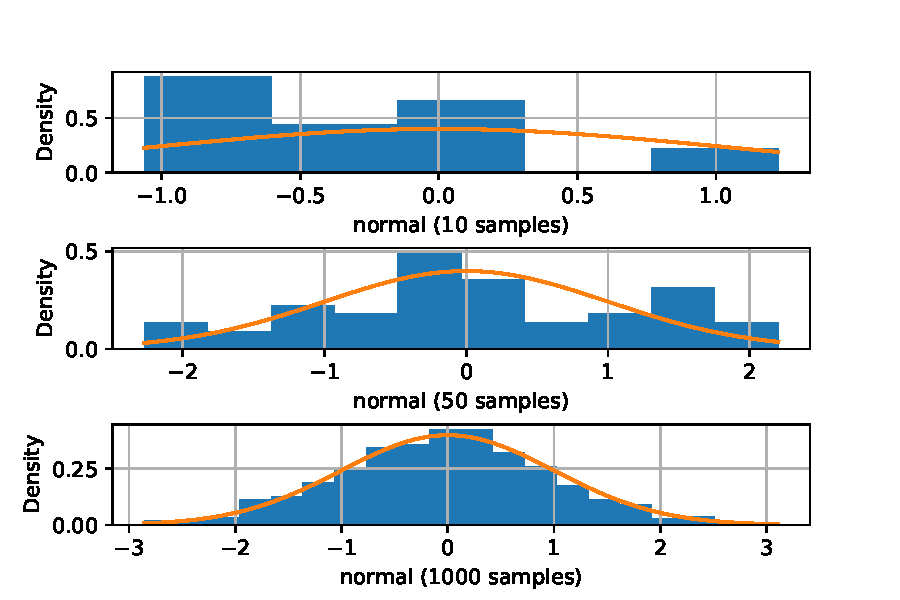
\includegraphics[width = 16 cm]{src/normal}
            \caption{Нормальное распределение~\eqref{eq:norm}}
            \label{fig:norm}
        \end{figure}

        \begin{figure}[H]
            \centering
            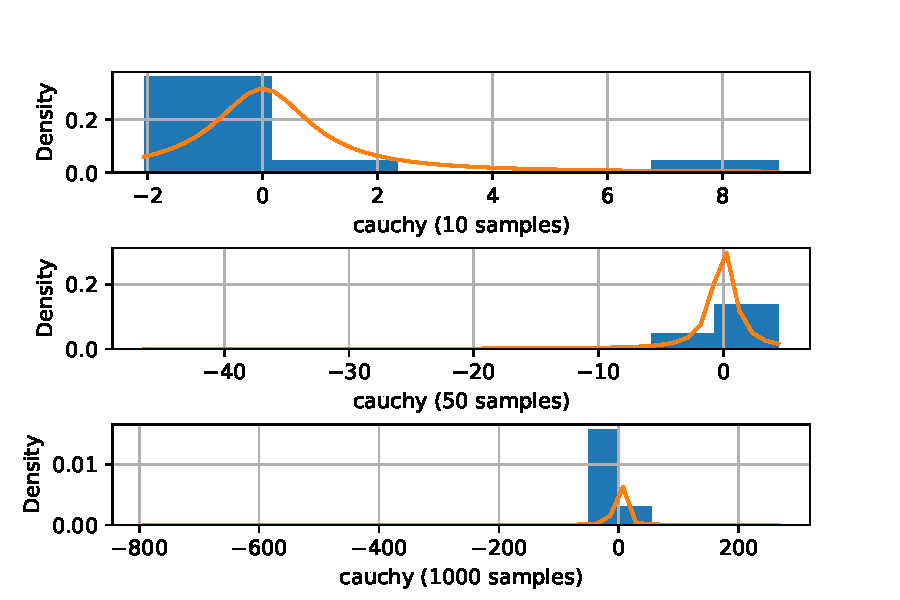
\includegraphics[width = 16 cm]{src/cauchy}
            \caption{Распределение Коши~\eqref{eq:cauchy}}
            \label{fig:cauchy}
        \end{figure}

        \begin{figure}[H]
            \centering
            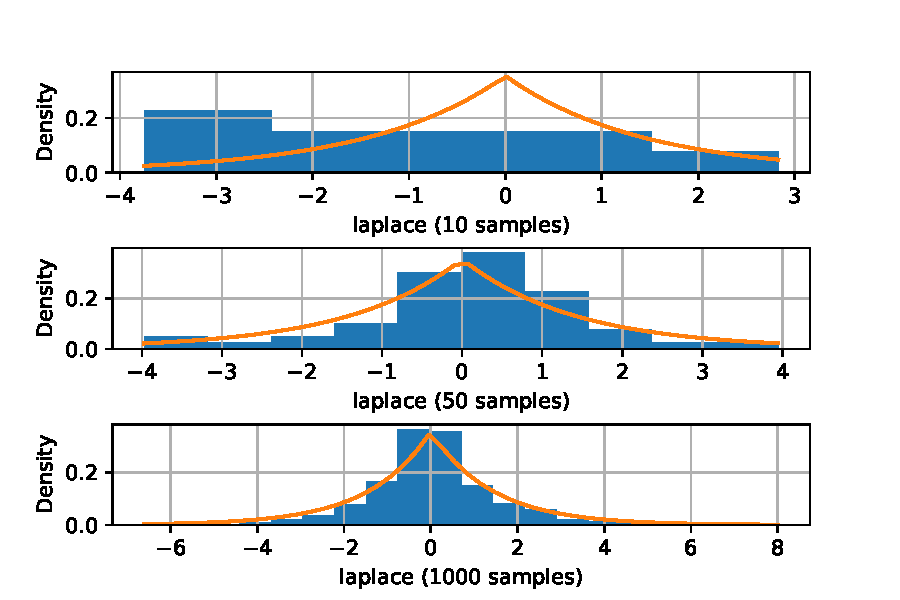
\includegraphics[width = 16 cm]{src/laplace}
            \caption{Распределение Лапласа~\eqref{eq:laplace}}
            \label{fig:laplace}
        \end{figure}

        \begin{figure}[H]
            \centering
            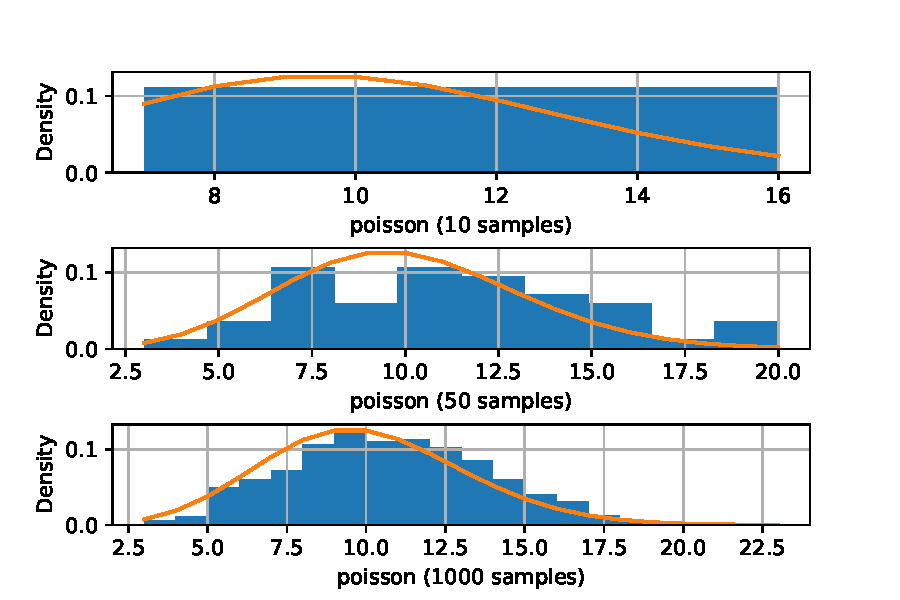
\includegraphics[width = 16 cm]{src/poisson}
            \caption{Распределение Пуассона~\eqref{eq:poisson}}
            \label{fig:poisson}
        \end{figure}

        \begin{figure}[H]
            \centering
            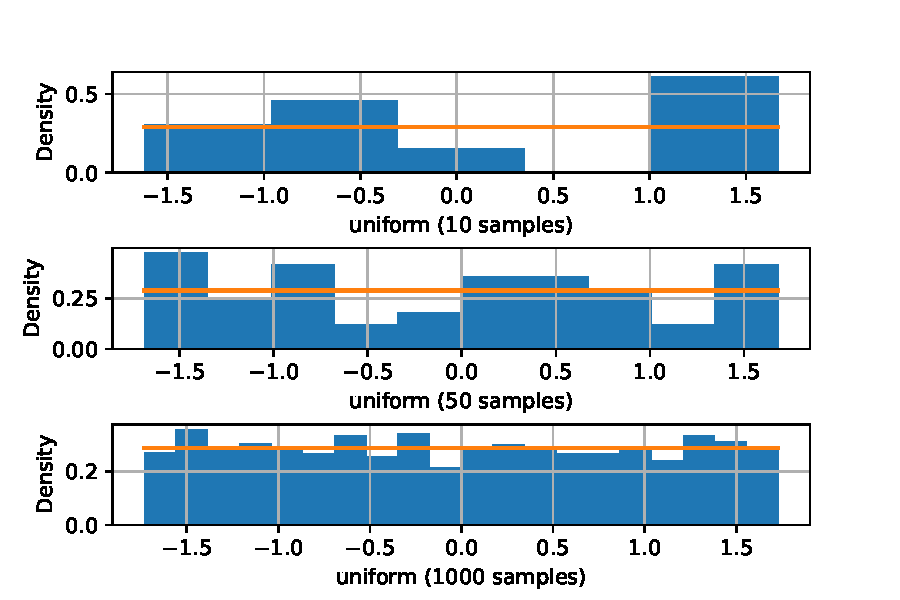
\includegraphics[width = 16 cm]{src/uniform}
            \caption{Равномерное Распределение~\eqref{eq:uniform}}
            \label{fig:uniform}
        \end{figure}

    \section{Обсуждение}
        Видно, что во всех рассмотренных случаях при увеличении размера выборки гистограмма приближается к графику функции плотности вероятности закона, по которому распределены элементы.
        При малом размере выборки невозможно понять по какому распределению генерировалась выборка так как все гистограммы похожи друг на друга.
    \section*{Примечание}
        С кодом работы и отчета можно ознакомиться по ссылке:\;\url{https://github.com/sqrtyyy/MathStat/tree/master/lab_1}
\end{document}